% async-a-sync -- beamer slides
% Compile:  pdflatex presentation.tex
% Numbers are freshly measured on this repo's NVMe with demos/demo_wordcount.c,
% 512 files x 4 KiB, page cache dropped. One source built three ways:
%   gcc sync ~22 ms | Fil-C sync ~25 ms | Fil-C implicit ~13 ms.
% Fil-C baseline overhead vs gcc here is ~1.1x; implicit is ~2.0x over Fil-C
% sync and ~1.7x over gcc sync. Ratios vary a bit run to run.

\documentclass[aspectratio=169]{beamer}

\usetheme{Madrid}
\usecolortheme{default}
\setbeamertemplate{navigation symbols}{}
\setbeamertemplate{footline}{\hfill\insertframenumber/\inserttotalframenumber\kern1em}

\usepackage[T1]{fontenc}
\usepackage{listings}
\usepackage{booktabs}
\usepackage{graphicx}
\usepackage{tikz}
\usetikzlibrary{positioning,arrows.meta,fit,backgrounds}

\lstset{
  language=C,
  basicstyle=\ttfamily\scriptsize,
  keywordstyle=\color{blue!70!black}\bfseries,
  commentstyle=\color{green!40!black},
  stringstyle=\color{red!70!black},
  numbers=none,
  frame=single,
  rulecolor=\color{black!20},
  columns=fullflexible,
  keepspaces,
  showstringspaces=false,
  aboveskip=4pt,
  belowskip=4pt,
}

\title{async-a-sync}
\subtitle{Transparent asynchronous syscalls on Fil-C}
\author{}
\date{}

\begin{document}

\begin{frame}
  \titlepage
\end{frame}

% ==================================================================
\begin{frame}{The basic idea}
  Make syscalls asynchronous \textbf{without changing the call site}. The call
  site is ordinary C; the runtime adds the overlap underneath.

  \begin{block}{Three mechanisms working together}
    \begin{enumerate}
      \item \textbf{Non-blocking submission.}
        A syscall becomes an \texttt{io\_uring} entry; the call returns without waiting.
      \item \textbf{Provenance-tracked results.}
        The returned value carries a tag naming its pending request; anything
        derived from it inherits that tag.
      \item \textbf{Resolution on first real access.}
        The first use checks the completion queue: if the request has landed,
        the access proceeds; otherwise the caller waits.
    \end{enumerate}
  \end{block}
\end{frame}

% ==================================================================
\begin{frame}{Where the hook goes: Fil-C already checks every access}
  Fil-C provides most of the machinery.

  \begin{itemize}
    \item Every pointer carries an \textbf{invisible capability}: bounds and
      type, stored out of band.
    \item \texttt{FilPizlonator} transforms every pointer operation into a
      dynamic capability check.
    \item There is \textbf{no escape hatch}: no \texttt{unsafe}, and no unsafe
      code can be linked outside a small trusted core.
    \item Syscalls are already a checked boundary, routed through \texttt{libpizlo}.
  \end{itemize}

  \vspace{4pt}
  Consequently we do not add a second instrumentation pass. We extend the check
  that is already on every access.
\end{frame}

% ==================================================================
\begin{frame}{InvisiCaps: how Fil-C tracks provenance}
  A pointer's \textbf{capability} (bounds and type) is stored \emph{out of
  band} from its bits. Propagating the pointer therefore propagates the tag, not
  just an address.

  \begin{center}
  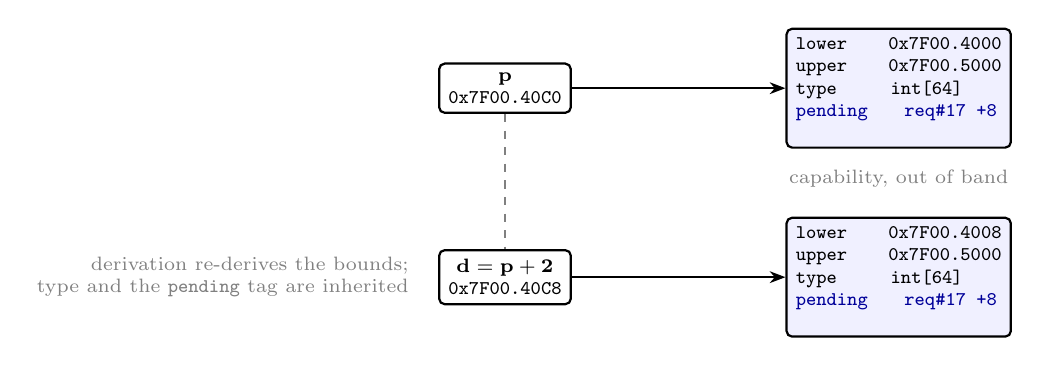
\begin{tikzpicture}[
      /tikz/font=\scriptsize,
      ptrbox/.style={draw, rounded corners=2pt, thick, fill=white, align=center},
      capbox/.style={draw, rounded corners=2pt, thick, fill=blue!6, align=left},
      thickarr/.style={-{Stealth[length=2mm]}, thick},
    ]
    % p and its capability
    \node[ptrbox] (p) at (0,0) {$\mathbf{p}$\\\texttt{0x7F00.40C0}};
    \node[capbox] (c1) at (5.0,0) {
      \texttt{lower\quad\;\: 0x7F00.4000}\\
      \texttt{upper\quad\;\: 0x7F00.5000}\\
      \texttt{type\quad\;\;\;\; int[64]}\\
      {\color{blue!60!black}\texttt{pending\;\;\;\;\, req\#17 +8}}\\
    };
    \draw[thickarr] (p) -- (c1);
    \node[below=0.15cm of c1, text=gray] {capability, out of band};

    % d = p + 2 and its capability
    \node[ptrbox] (d) at (0,-2.4) {$\mathbf{d = p + 2}$\\\texttt{0x7F00.40C8}};
    \node[capbox] (c2) at (5.0,-2.4) {
      \texttt{lower\quad\;\: 0x7F00.4008}\\
      \texttt{upper\quad\;\: 0x7F00.5000}\\
      \texttt{type\quad\;\;\;\; int[64]}\\
      {\color{blue!60!black}\texttt{pending\;\;\;\;\, req\#17 +8}}\\
    };
    \draw[thickarr] (d) -- (c2);

    \draw[gray, dashed, thick] (p) -- (d);
    \node[left=0.25cm of d, text=gray, align=right]
      {derivation re-derives the bounds;\quad\\type and the \texttt{pending} tag are inherited};
  \end{tikzpicture}
  \end{center}

  \begin{itemize}
    \item \texttt{FilPizlonator} already turns every pointer operation into a
      dynamic capability check; that check is the hook point.
    \item The runtime records, for an async result, which pending request fills
      it (a request id and an offset). Resolution clears the pending bit in
      place; the address itself never changes, because the kernel was already
      given the destination.
  \end{itemize}
\end{frame}

% ==================================================================
\begin{frame}{Provenance $\rightarrow$ lazy values}
  A pending value carries a \textbf{request id} (and an offset). It is not ready
  until that request completes.

  \begin{block}{What ``using'' it means}
    \begin{itemize}
      \item Dereference, field access, and indexing all go through the
        capability check Fil-C already emits.
      \item That check calls \texttt{filc\_resolve\_pending} first.
      \item Resolution clears the \textbf{pending bit in place}: the buffer
        address never changes, because the kernel was already given the
        destination.
    \end{itemize}
  \end{block}

  \begin{itemize}
    \item Fast path: \textbf{one acquire load}; if nothing is in flight, return.
    \item Slow path: find the covering request, \textbf{spin} against the
      completion ring in userspace, \textbf{park} only if it has not landed.
  \end{itemize}

  \small This is the same shape as Brooks forwarding pointers and GHC thunk
  blackholing: a check before access, with self-healing update.
\end{frame}

% ==================================================================
\begin{frame}[fragile]{Dependent syscalls: how they are resolved}
  Three cases. Two of them are free, discovered from ordinary dataflow.

  \small
  \begin{block}{Explicit dataflow: no annotation is required}
    \texttt{x = a();\; b(x):} the pending tag on \texttt{a}'s result \emph{is}
    the dependency edge, discovered from ordinary dataflow. Both requests are
    submitted immediately; only the first \emph{access} into \texttt{a}'s result
    blocks.
  \end{block}

  \begin{block}{The same fd: sharing it is the dependency}
    A provenant value of type \texttt{fd} is just like any other: it names the
    pending request that produced it student. Two operations that take the
    \emph{same} fd therefore share that tag, and the second resolves the first:

    \begin{lstlisting}[aboveskip=2pt,belowskip=0pt]
fd = fasync_open_pending(path);   /* async, pending tag on fd */
fasync_pread(fd, ...);            /* waits for open */
fasync_pwrite(fd, ...);           /* waits for pread */
    \end{lstlisting}

    Nothing is declared: the shared value \emph{is} the edge, exactly as for any
    other type. The fd cannot be used before it exists, and every operation that
    touches it keeps the batch one request behind the previous one.
  \end{block}

  \begin{block}{Descriptors: just like before, for values of type fd}
    An async \texttt{openat} cannot return an fd that does not exist yet.
    \texttt{fasync\_open\_pending} instead returns a \textbf{pending descriptor}
    (negative, so it can never collide with a real fd), and every operation that
    takes an fd resolves it first. Passing the pending descriptor to
    \texttt{fasync\_pread} \emph{is} the dependency: nothing is declared, nothing is
    remembered.
  \end{block}

  \small
  Resolution is the same machinery as any pending value: find the covering request,
  \textbf{spin} against the completion ring, \textbf{park} only if it has not
  landed. Kernel-native chaining (\texttt{IOSQE\_IO\_LINK} + direct descriptors)
  would hand the ordering to the kernel; this kernel does not honour an explicit
  \texttt{openat} slot (\texttt{stage6b}), so ordered in userspace.
\end{frame}

% ==================================================================
\begin{frame}{Hidden dependencies: declared by the programmer}
  When two operations share no value in the source but touch the same memory, path,
  or fd, dataflow cannot see the edge, so the programmer must declare it.

  \small
  \begin{block}{The token formulation}
    Every async call takes a hidden trailing \texttt{void* PROVENANCE} argument.
    The programmer writes \texttt{void* t = prov\_alloc();} and passes \texttt{t} to
    every call that must be ordered against the others sharing it.
  \end{block}

  \begin{block}{Here: declared effect sets, with a capability proof}
    Each operation declares what it reads and writes (\texttt{FASYNC\_IN / OUT /
    INOUT}); the dependency DAG falls out. Before falling back to the declarations,
    the analyser \textbf{proves operands disjoint} from their InvisiCap bounds
    (\texttt{zgetlower}/\texttt{zgetupper}); conflicting-looking kinds still run
    concurrently when the objects provably do not overlap. Tokens are a named
    resource claimed \texttt{INOUT}.
  \end{block}

  \vspace{-4pt}
  \begin{columns}[T]
    \begin{column}{0.40\textwidth}
      \tiny
      \begin{tabular}{@{}lrr@{}}
        \toprule
        encoding & edges & in flight \\
        \midrule
        effect sets & 4 & 5 \\
        two tokens & 6 & 2 \\
        one token & 15 & 1 \\
        \bottomrule
      \end{tabular}
    \end{column}
    \begin{column}{0.55\textwidth}
      \small Six operations, two independent chains: a token expresses only a
      chain (everyone sharing it serializes against everyone), which is the
      over-serialization of the single-token row above.
    \end{column}
  \end{columns}
\end{frame}

% ==================================================================
\begin{frame}{The substrate: \texttt{io\_uring}}
  The converse of FlexSC: \textbf{do not pay a context switch per operation;
  pay one per batch.}

  \begin{block}{The properties we rely on}
    \begin{itemize}
      \item \textbf{Batched submission:} many operations in one non-blocking
        \texttt{io\_uring\_enter}.
      \item \textbf{Completion in shared memory:} the completion queue is read
        from userspace, with no syscall to reap.
      \item \texttt{SQPOLL:} submission becomes a plain store, with no kernel
        entry at all.
    \end{itemize}
  \end{block}

  \vspace{4pt}
  One structural constraint: the ring must use \texttt{NO\_MMAP}. Fil-C's
  \texttt{mmap} cannot map an \texttt{io\_uring} ring (it forces
  \texttt{MAP\_FIXED}), so the caller supplies the ring memory itself.
\end{frame}

% ==================================================================
\begin{frame}{No submit: the batch publishes lazily}
  Enqueueing an operation does not reach the kernel. It writes an SQE into
  shared memory and bumps a counter; the kernel sees the work only once the SQ
  tail word is stored.

  Both resolution paths publish the whole queue on the first access that
  genuinely needs a completion:

  \begin{itemize}
    \item Memory-safe half: \texttt{fasync\_resolve\_pending} calls
      \texttt{fasync\_submit()}.
    \item Compiler-emitted hook: \texttt{filc\_resolve\_pending} calls
      \texttt{fasync\_native\_submit()}, which fills the SQ index array, stores
      the tail, and issues one non-blocking \texttt{io\_uring\_enter}.
  \end{itemize}

  \begin{block}{What is preserved}
    \begin{itemize}
      \item \textbf{Batching:} the whole queued workload publishes in one enter,
        not one syscall per operation.
      \item \textbf{Cheap fast path:} when nothing is pending, resolution stays
        one acquire load, and \texttt{fasync\_submit()} is a no-op on an empty
        queue.
      \item \textbf{No escape hatch:} the publish is native, the shape the
        compiler hook requires; the shared state lives in
        \texttt{fasync\_shared.h}.
    \end{itemize}
  \end{block}

  \small Verified by \texttt{stage2\_lazy\_submit}: 8 reads of 256 KiB, no
  \texttt{submit()} anywhere. \texttt{kernel\_submit\_entries} is 0 after
  enqueue and exactly 1 after the first access.
\end{frame}

% ==================================================================
\begin{frame}[fragile]{The same program, built two ways}

  \begin{lstlisting}
read_all_files();
for (i = 0; i < N; i++)
    words += wordcount(file_data(i));
  \end{lstlisting}

  One source file (\texttt{demos/demo\_wordcount.c}). A build flag selects the
  backend:
  \begin{itemize}
    \item \textbf{sync:} \texttt{read\_all\_files()} is a blocking
      \texttt{pread} loop.
    \item \textbf{implicit:} \texttt{read\_all\_files()} enqueues every read and
      returns; counting a file's buffer is what waits, and the first access
      publishes the whole queue lazily.
  \end{itemize}

  No submit, no wait, no marker exists anywhere in the program.
\end{frame}

% ==================================================================
\begin{frame}{Performance gains}
  Word count over \textbf{512 files $\times$ 4 KiB}, page cache dropped before
  each pass. Same source, three toolchains.

  \begin{center}
    \begin{tabular}{lr}
      \toprule
      toolchain & time \\
      \midrule
      gcc, sync        & $\sim$22 ms \\
      Fil-C, sync      & $\sim$25 ms \\
      Fil-C, implicit  & $\sim$13 ms \\
      \bottomrule
    \end{tabular}
  \end{center}

  \begin{itemize}
    \item Implicit vs Fil-C sync is $\approx$2.0$\times$; vs gcc sync,
      $\approx$1.7$\times$.
    \item Fil-C's own overhead here is $\approx$1.1$\times$ over gcc (the
      documented 1.5--4$\times$ is for heavier code, not this workload).
    \item No wait is written; the batch reaches the kernel in one lazy
      submission.
  \end{itemize}
\end{frame}

% ==================================================================
\begin{frame}{Ergonomics}
  The comparison is against ordinary synchronous C, the code a programmer would
  actually have written. Overlapping the reads is worth roughly \textbf{2$\times$}
  over the same source built with plain Fil-C, and \textbf{1.7$\times$} over the
  gcc build.

  \begin{itemize}
    \item No state machine, callback, poll loop, handle, or wait is written.
    \item No submit function exists: the queue is published when the first
      buffer is touched.
    \item The only difference between the arms is the build (compiler and
      flags): same source, same function.
  \end{itemize}

  \vspace{4pt}
  \begin{block}{Limits}
    With a warm page cache there is nothing to overlap and no win. This disk
    sustains $\sim$184 kIOPS; the runtime currently reaches $\sim$52 kIOPS; the
    remaining gap is an \texttt{io-wq} concurrency ceiling, not the design.
  \end{block}
\end{frame}

% ==================================================================
\begin{frame}[fragile]{Caveats}
  \begin{block}{Fil-C is the bet and the ceiling}
    \begin{itemize}
      \item \textbf{Young and single-maintainer.} One person owns the compiler,
        and it still pays a baseline: documented at 1.5--4$\times$ slower than
        gcc on general code. On this workload it measured $\approx$1.1$\times$.
      \item \textbf{No escape hatch.} Nothing unsafe can link outside a small
        trusted runtime, which is exactly where all this machinery has to live.
    \end{itemize}
  \end{block}

  \begin{block}{Hidden dependencies still need the programmer}
    The free case is dataflow: when \texttt{b} reads \texttt{a}'s result, no
    annotation is required. When two operations share no value but secretly
    touch the same memory, path, or fd, the dependency has to be declared with
    an effect set or a token:

    \begin{lstlisting}[aboveskip=2pt,belowskip=0pt]
void* t = prov_alloc();          /* manual ordering */
a(..., t);
b(..., t);            /* must run after a */
    \end{lstlisting}
    That declaration is the one thing a programmer must remember to write.
  \end{block}
\end{frame}

% ==================================================================
\begin{frame}{Limitations}
  \begin{itemize}
    \item \textbf{Supported ops are a subset.} \texttt{pread}, \texttt{pwrite},
      \texttt{openat}, \texttt{close}, \texttt{fsync}. Plain \texttt{read} is
      deliberately out: it has no offset, so its result depends on the file
      cursor at execution time, not submission time.
    \item \textbf{One ring, one lock.} Multi-threaded use is not tested; the
      collector handshake under concurrent blocking submits has not been
      reasoned through.
    \item \textbf{Kernel-native chaining is blocked here.} Dependent operations
      are ordered in userspace (\texttt{IOSQE\_IO\_LINK} + direct descriptors
      are not honoured by this kernel).
    \item \textbf{The device's parallelism is not fully reached.} The implicit
      path runs at $\sim$52 kIOPS where plain blocking threads sustain
      $\sim$184 kIOPS; the gap is an \texttt{io-wq} worker ceiling, not the
      design.
    \item \textbf{Aliasing writes are not tracked.} A write into a pending
      buffer that bypasses the checked access path would race with the kernel.
  \end{itemize}
\end{frame}

% ==================================================================
\begin{frame}{Recap}
  \begin{enumerate}
    \item Fil-C's per-access capability check is the hook point; no separate
      instrumentation pass is needed.
    \item A pending value resolves at first use; provenance and submission are
      both lazy.
    \item \texttt{io\_uring} supplies the overlap; the compiler supplies the
      transparency.
    \item Same source, same function, $\approx$2$\times$ over plain Fil-C and
      $\approx$1.7$\times$ over gcc on uncached I/O.
  \end{enumerate}
\end{frame}

% ==================================================================
\begin{frame}{Future scope}
  \begin{itemize}
    \item \textbf{Pluggable completion backends.} The resolution machinery only
      needs something to poll. Make the backend an interface (\texttt{io\_uring}
      today; sockets, timers, RDMA later), selected \emph{per function} rather
      than globally, riding on the existing effect-set annotation.
    \item \textbf{Core pinning for cache locality.} The resolution path owns hot
      state: the request table, the completion ring, the in-flight flag. Pinning
      the functions that touch it to fixed cores would avoid cross-core traffic
      on every resolve.
    \item \textbf{Fold resolution into the bounds check.} A pending bit in the
      InvisiCap makes an access cost one compare instead of a call to
      \texttt{filc\_resolve\_pending}. When no batch is in flight the call is
      already one load; this targets the per-access cost while a batch runs.
    \item \textbf{Close the device-parallelism gap.} Raise the \texttt{io-wq}
      worker ceiling to reach the concurrency the device demonstrably sustains.
  \end{itemize}
\end{frame}

\end{document}